%%%%%%%%%%%%%%%%%%%%%%%%%%%%%%%%%%%%%%%%%%%%%%%%%%%%%%%%%%%%%%%%%
\chapter{CHEST X-RAY}\label{ch:CH2}
%%%%%%%%%%%%%%%%%%%%%%%%%%%%%%%%%%%%%%%%%%%%%%%%%%%%%%%%%%%%%%%%%

X-radiations (X-rays) are electromagnetic waves which is actually a type of radiation. German physicist Wilhelm Konrad Röntgen discovered these specific type of photons while investigating cathode rays in Crookes tubes at 1895. Röntgen named these rays as X-radiations to signify an unknown type of radiation.

The first use of X-rays for chest imaging dates back to 1896. Nowadays, X-rays are mostly used in medical industry for medical and radiological imaging, and at public areas in purpose of security. 

The least photons are absorbed by air while the most photons are absorbed by the calcium in bones. That is why bones are visible as white. Fat and other soft tissues absorbs X-rays in middle level, so they are seen as gray. Because of the absorption properties of X-rays, stated above, the lungs are observed in blackish color.

\begin{figure}[h]
    \centering
    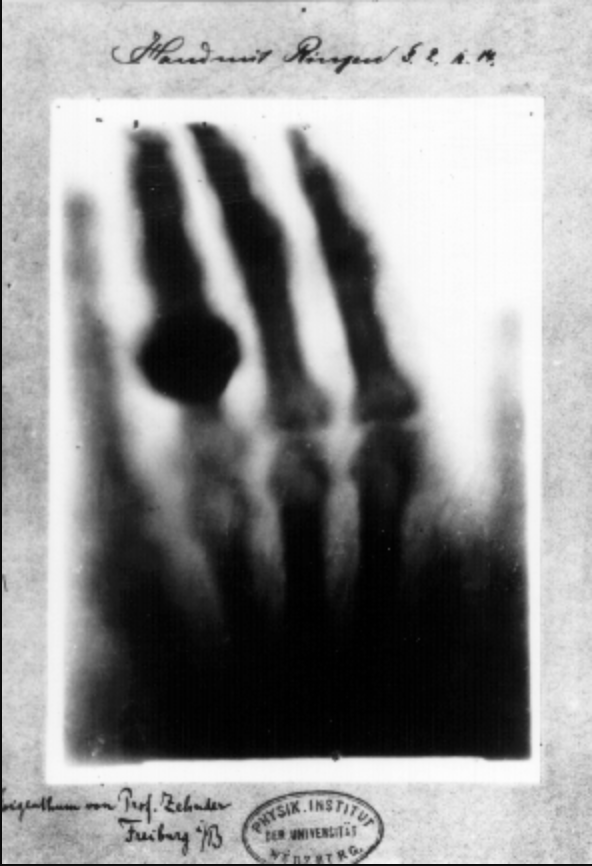
\includegraphics[keepaspectratio=true, scale=0.5]{./fig/first_medical_xray}
    % sekil2.eps: 0x0 pixel, 300dpi, 0.00x0.00 cm, bb=14 14 818 556
    \vspace*{3mm}
    \caption{Hand mit Ringen (Hand with Rings): print of Wilhelm Röntgen's first "medical" X-ray, of his wife's hand \cite{HandMitRingen}.}
    \label{fig:first_medical_xray}
\end{figure}

Chest X-rays can be taken in 3 main projection methods. The projection method may vary from country to country or even from hospital to hospital. However, the most preferred projection method is Postero-Anterior (PA) view in which X-rays go through from patient's posterior to anterior. The patient has to be stand during the operation. Second most used method is Antero-Posterior (AP) erect view. On the contrary of frontal view, beams traverse from anterior to posterior in AP projection.
When the PA or AP view is not possible due to the health issue of patient, such that the patient is not able to stay erect, supine position is applied as AP-Supine projection method. The other most used view type is Lateral (L) projection. It is performed from the left lateral of patient while the patient is standing. There are another various projection methods to film the chest of patient by X-rays.

\begin{figure}[h]
	\centering
	\subfigure[PA Projection]{\label{fig:chest_projections_a}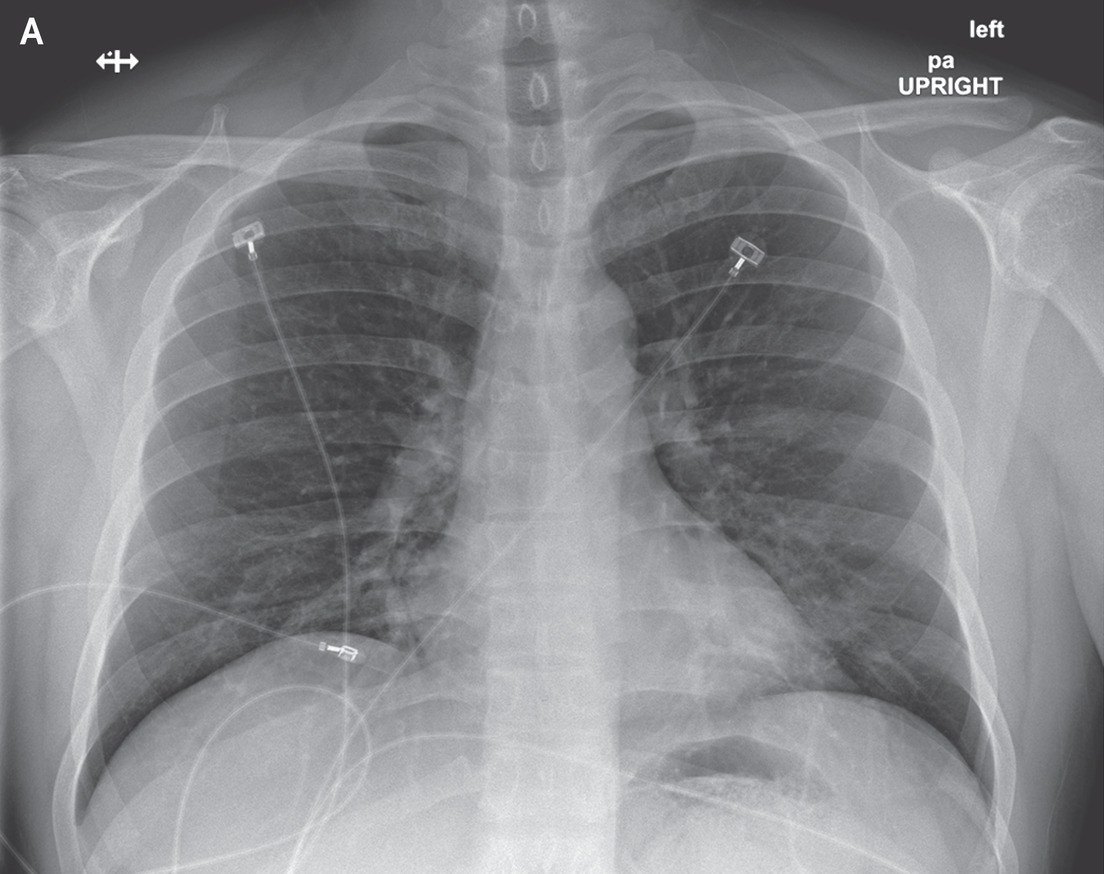
\includegraphics[width=.4\linewidth,height=.4\linewidth,scale=0.6]{chest_xray_PA}}
	\subfigure[AP Projection]{\label{fig:chest_projections_b}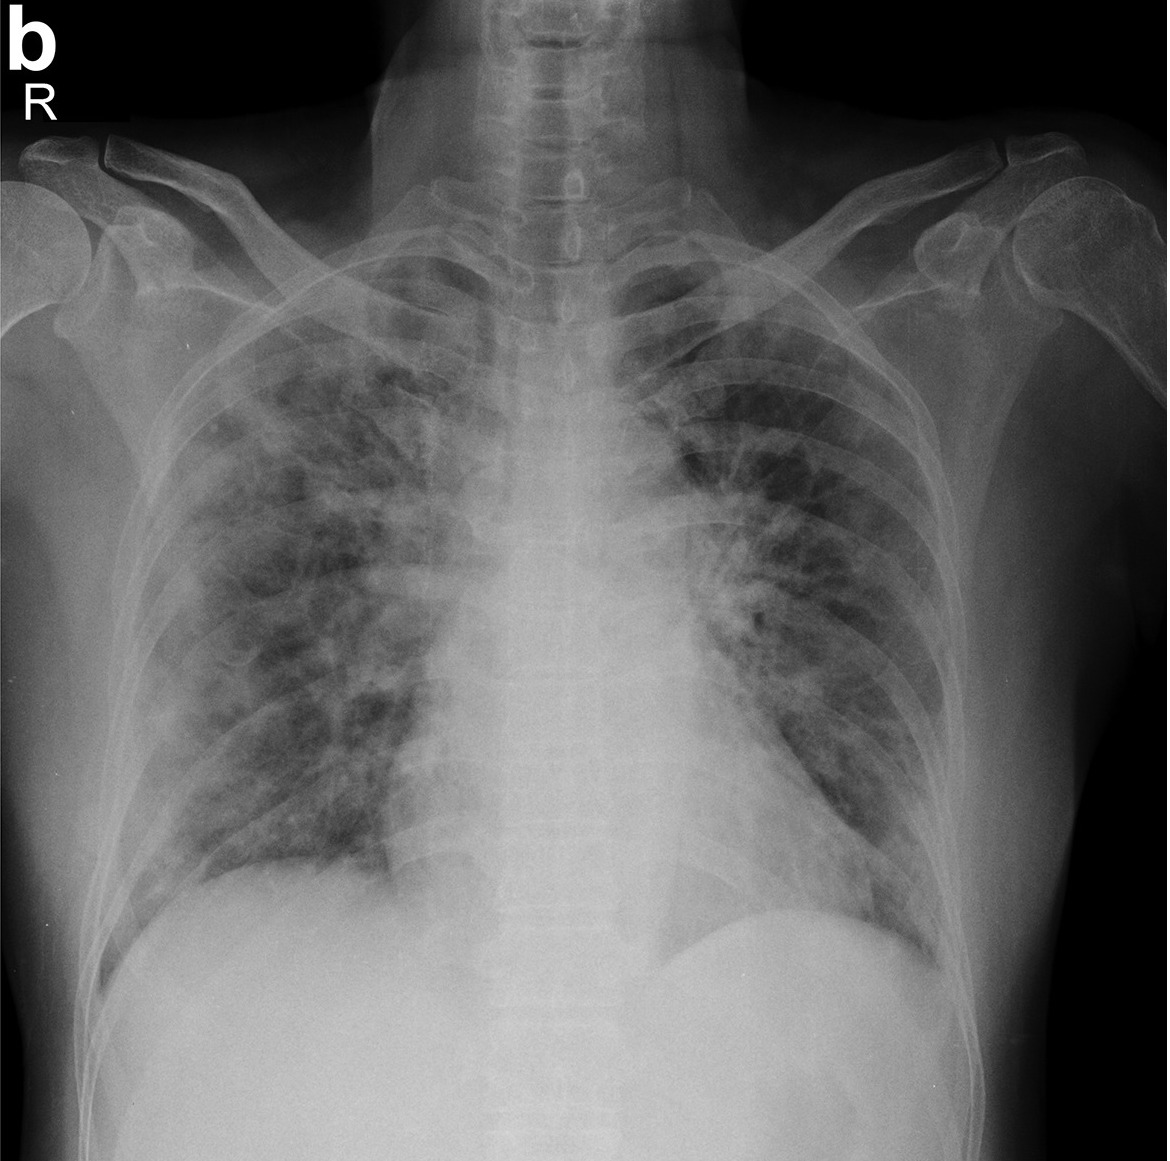
\includegraphics[width=.4\linewidth,height=.4\linewidth,scale=0.6]{chest_xray_AP}}
	\subfigure[AP Supine Projection]{\label{fig:chest_projections_c}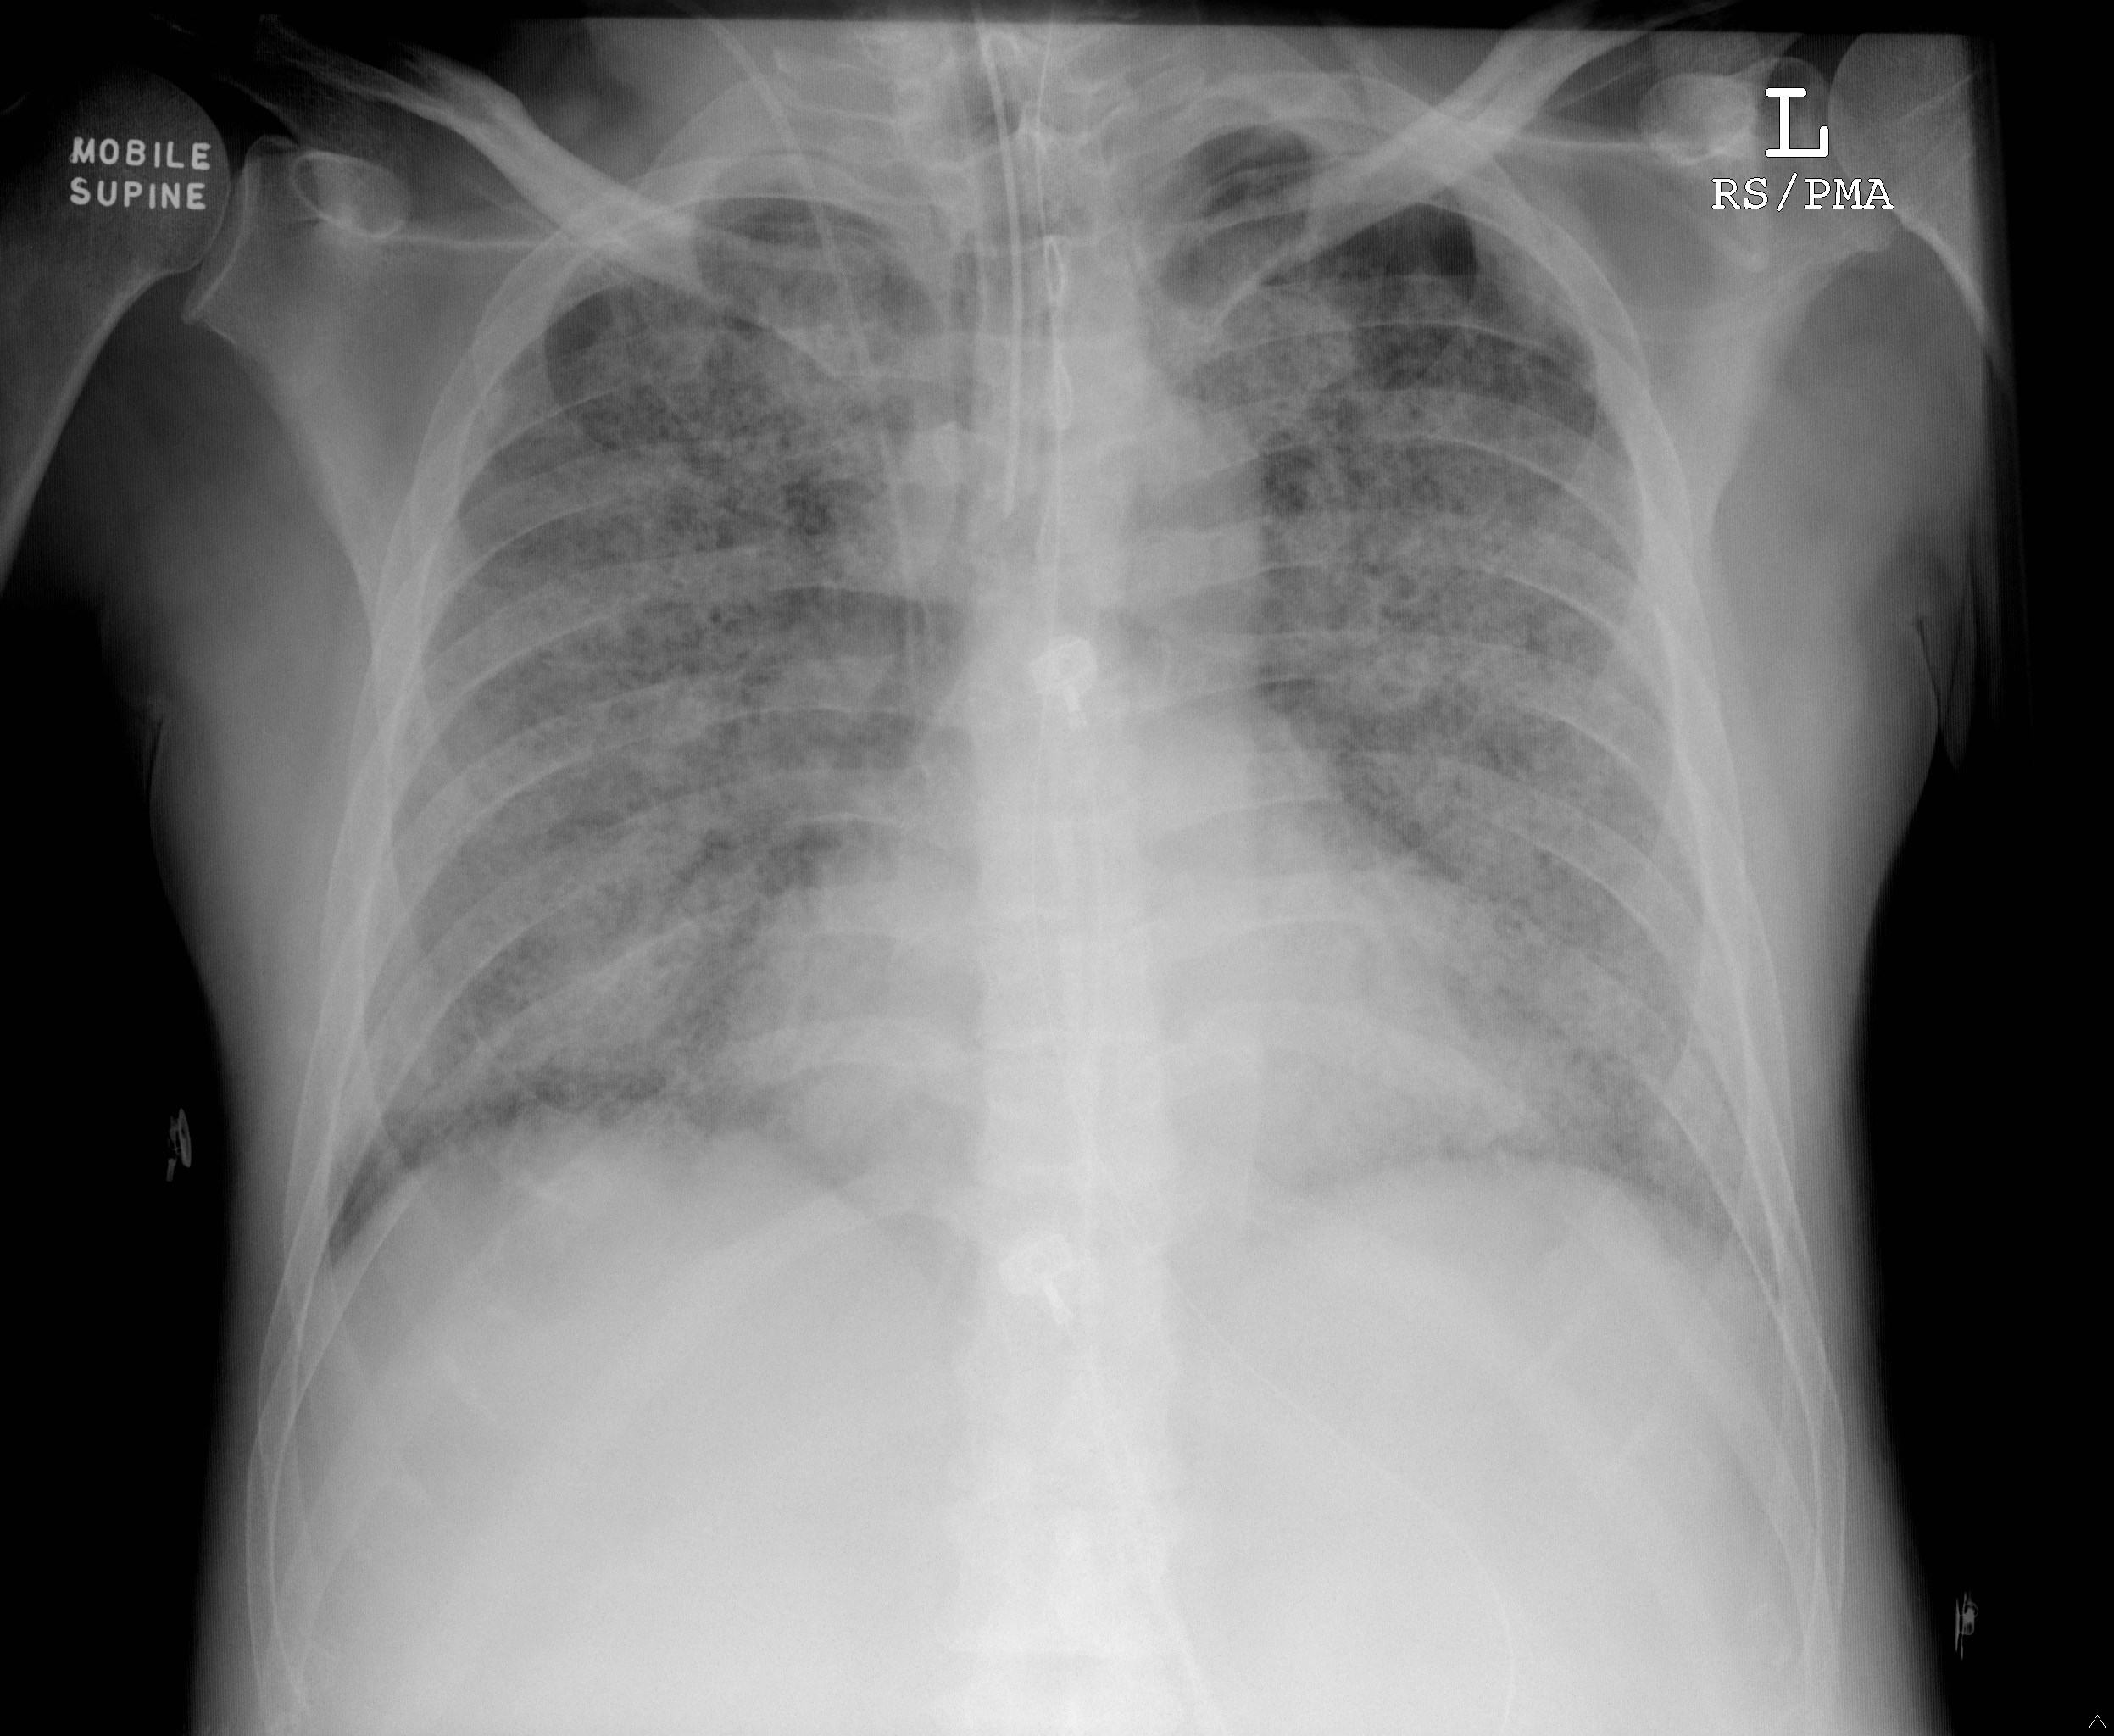
\includegraphics[width=.4\linewidth,height=.4\linewidth,scale=0.6]{chest_xray_AP_Supine}}
	\subfigure[L Projection]{\label{fig:chest_projections_d}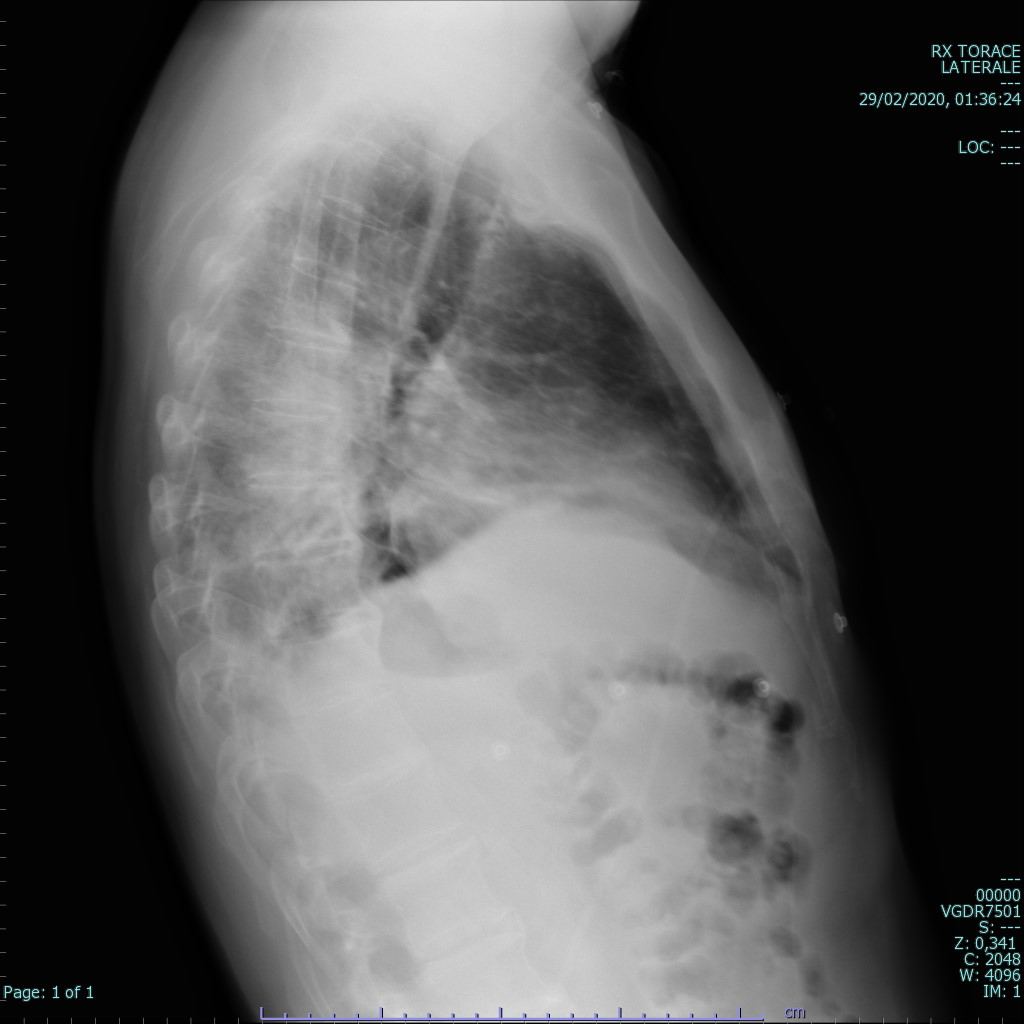
\includegraphics[width=.4\linewidth,height=.4\linewidth,scale=0.6]{chest_xray_L}}
	\captionfootnotemark{Chest X-Ray Projections.}
	\label{chest_projections}
\end{figure}
\footnotetext{Retrieved from GitHub: \hyperrefurl{https://github.com/ieee8023/covid-chestxray-dataset/tree/master/images} on March 25, 2021.}

Chest X-ray imaging has very significant role on detecting serious disease such as pneumonia and its causes, pneumothorax, heart failures, emphysema, lung cancer, broken ribs for years, and COVID-19 recently. Thanks to the accessibility and the ease of use of chest X-rays, various artificial intelligence problems can be formed and accomplished for the benefit of medical use, computer science and mathematics.
